\input ../SlidePreamble
\input ../preamble


\begin{document}

{\Huge
  \centerline{\bf TTIC 31230,  Fundamentals of Deep Learning}
  \vfill
  \centerline{David McAllester, Autumn   2021}
  \vfill
  \centerline{\bf Mutual Information Coding}
  \vfill
  \vfill

\slideplain{Mutual Information Coding}
\centerline{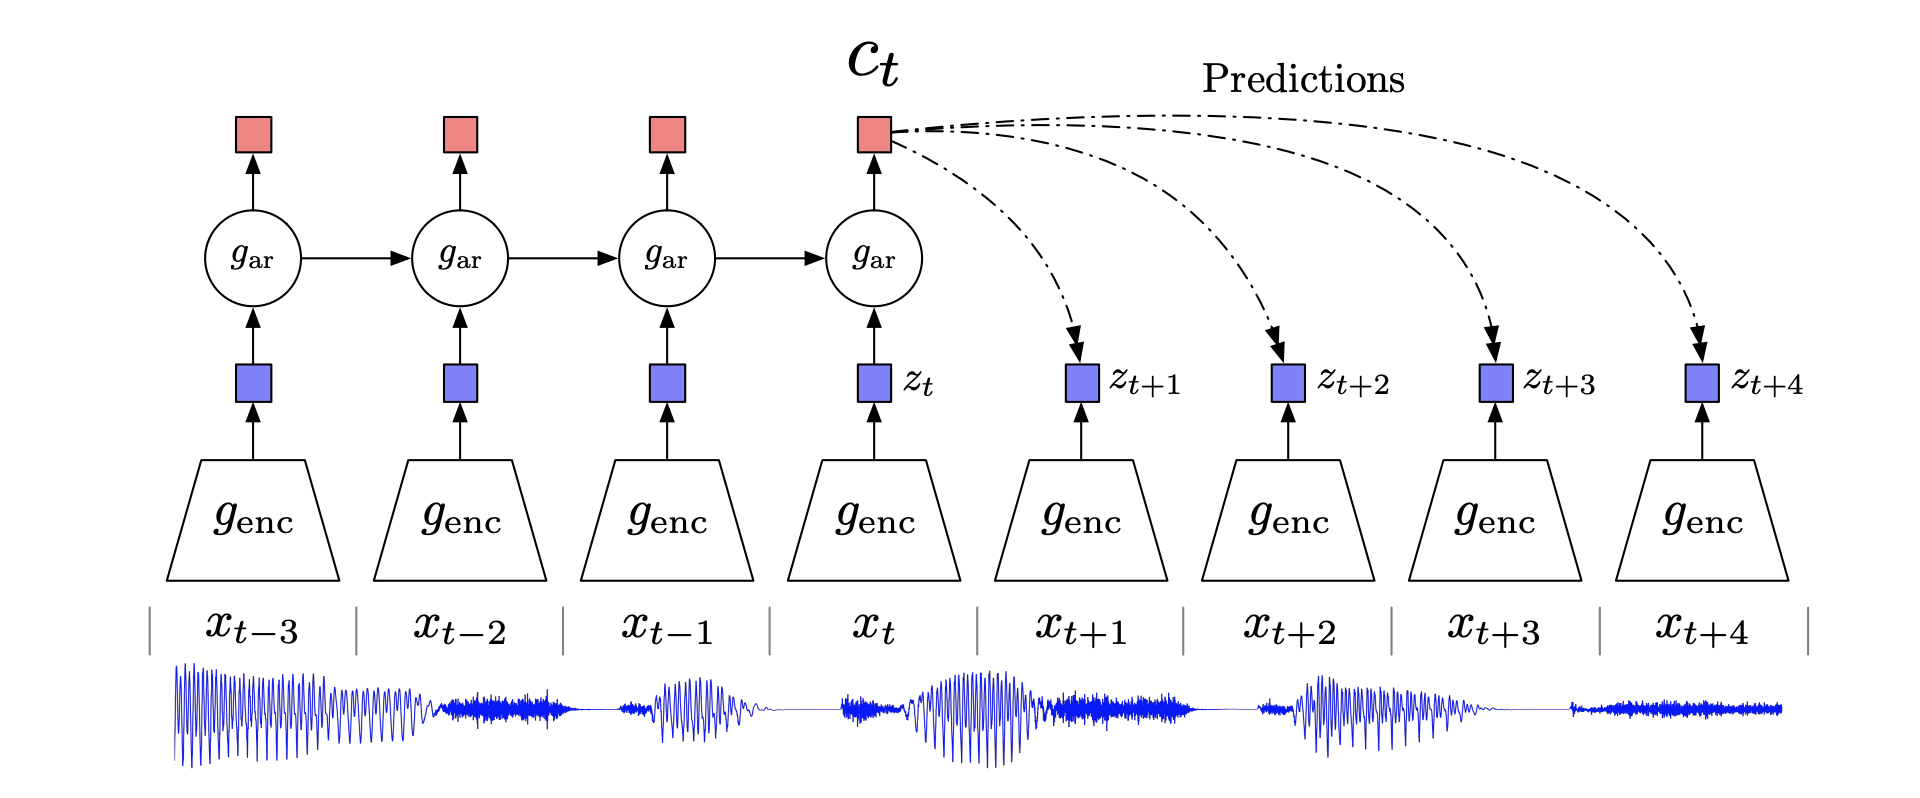
\includegraphics[width = 6 in]{\images/CPC}}
\centerline{\huge van den ORD et al. 2018}

\vfill
Consider the problem of learning phonetic representations of speech sounds.  In the figure each $z_t$ is a symbol representing the sound at time $t$.


\slideplain{Mutual Information Coding}
\centerline{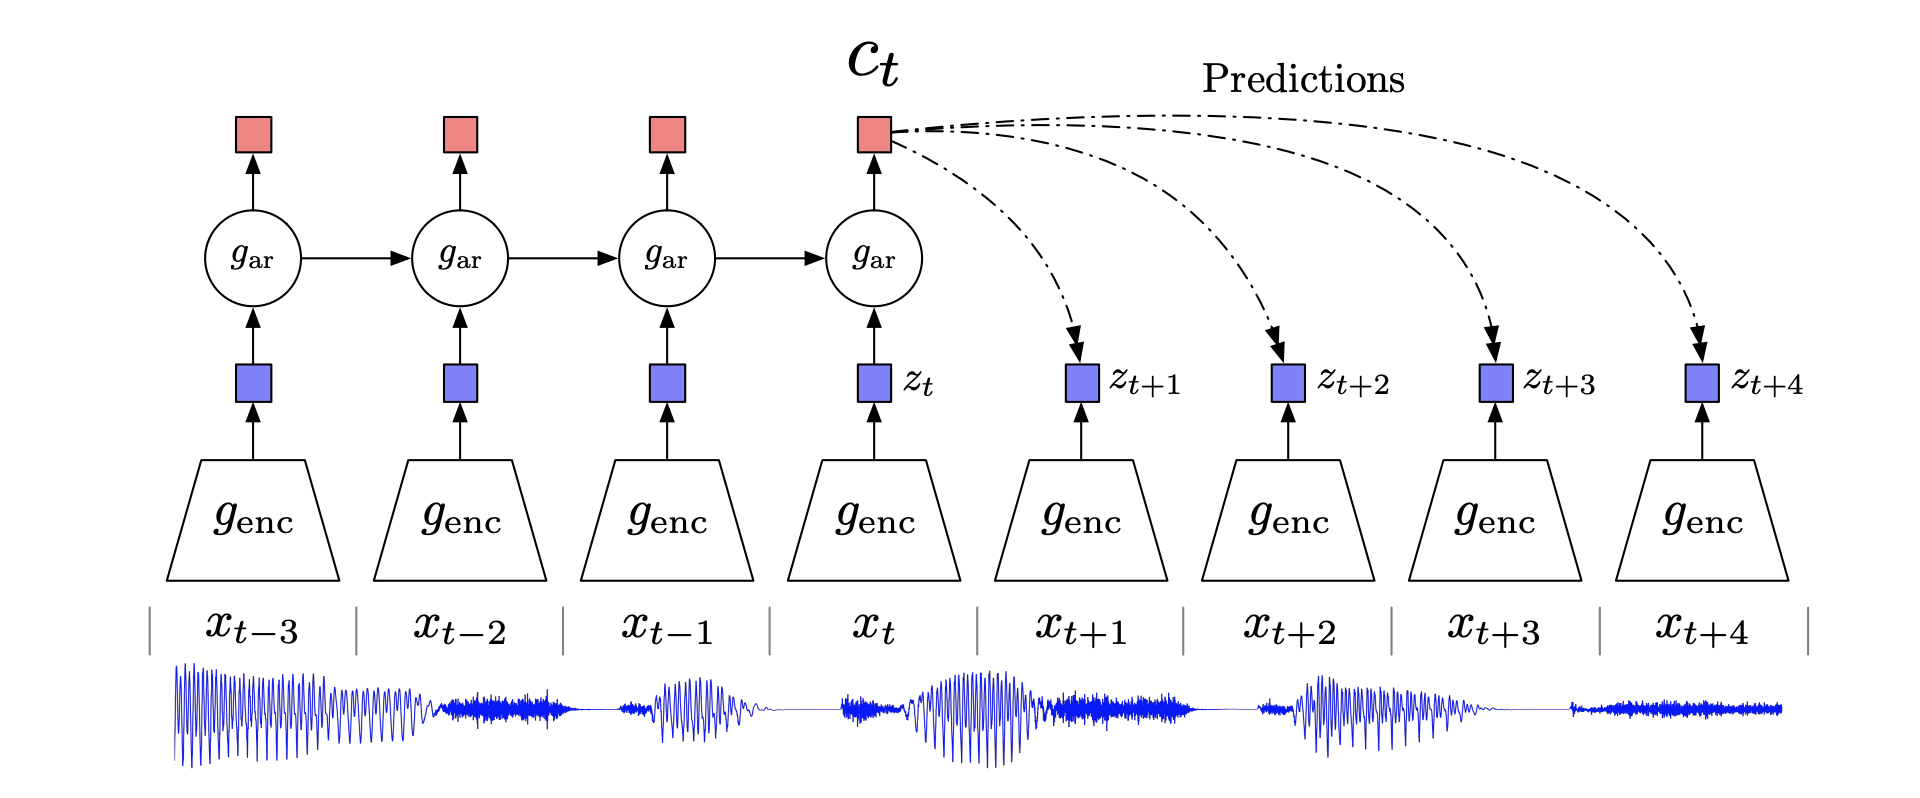
\includegraphics[width = 6 in]{\images/CPC}}
\centerline{\huge van den ORD et al. 2018}

\vfill
{\bf Unlike VAEs}, mutual information coding is about {\bf predicting latent variables}. There is no attempt to model the input speech sound.
Intuitively we want to separate signal from noise and avoid modeling noise.

\slide{wav2vec 2.0}

\vfill
Trained on 53k hours of {\bf unlabeled} audio they convert speech to a sequence of symbols they call ``pseudo-text units''.

\vfill
Using this pre-trained transcription of speech into pseudo-text they reduce the amount of labeld data needed for a given accuracy in speech recognition by a factor of 100.

\vfill
\centerline{\huge Baevski et al., 2020}

\slide{SwAV}

Mutual information coding as pretraining of image features.

\centerline{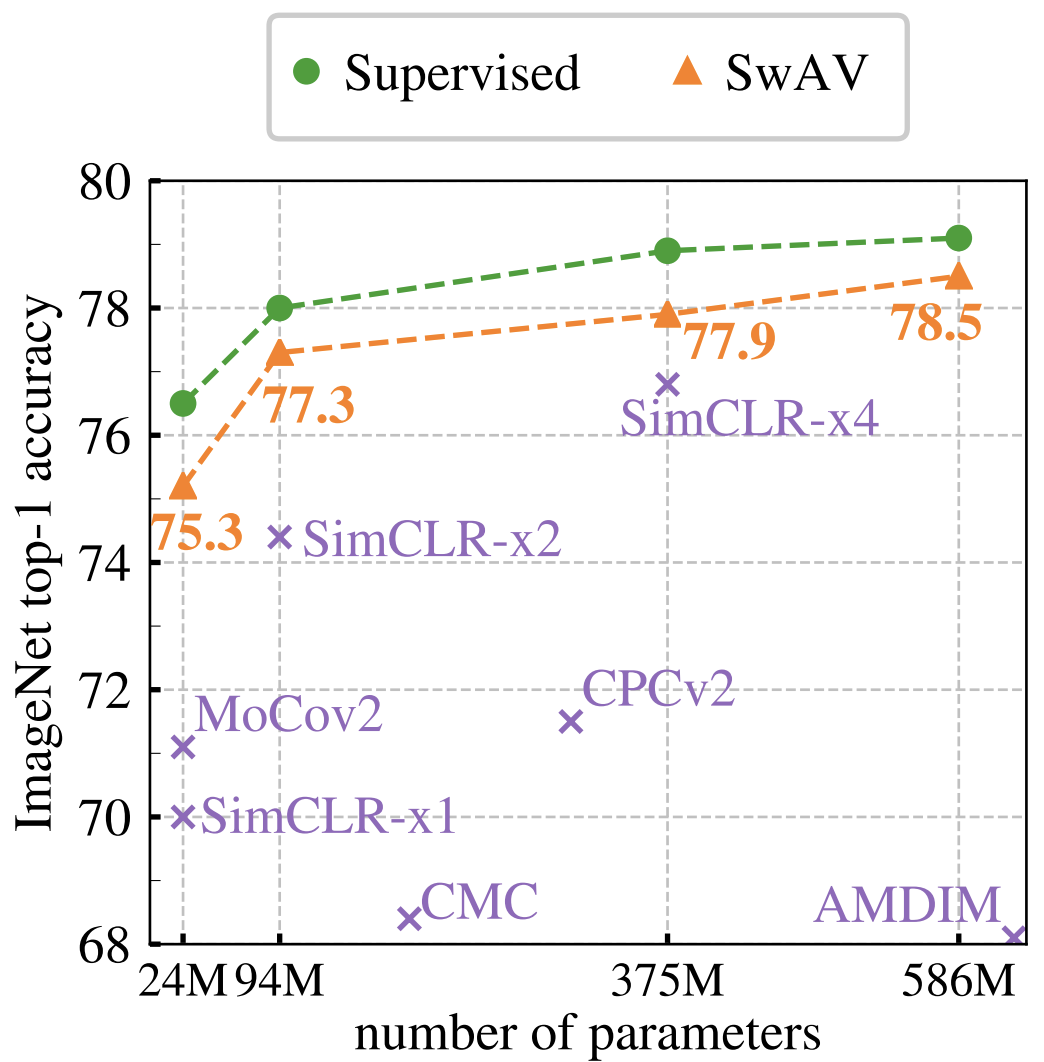
\includegraphics[width = 4.0in]{\images/SwAV}}

\centerline{\huge Caron et al. 2021}


\slide{Mutual Information Coding: General Formulation}

\centerline{$z_x$~~~~}
\centerline{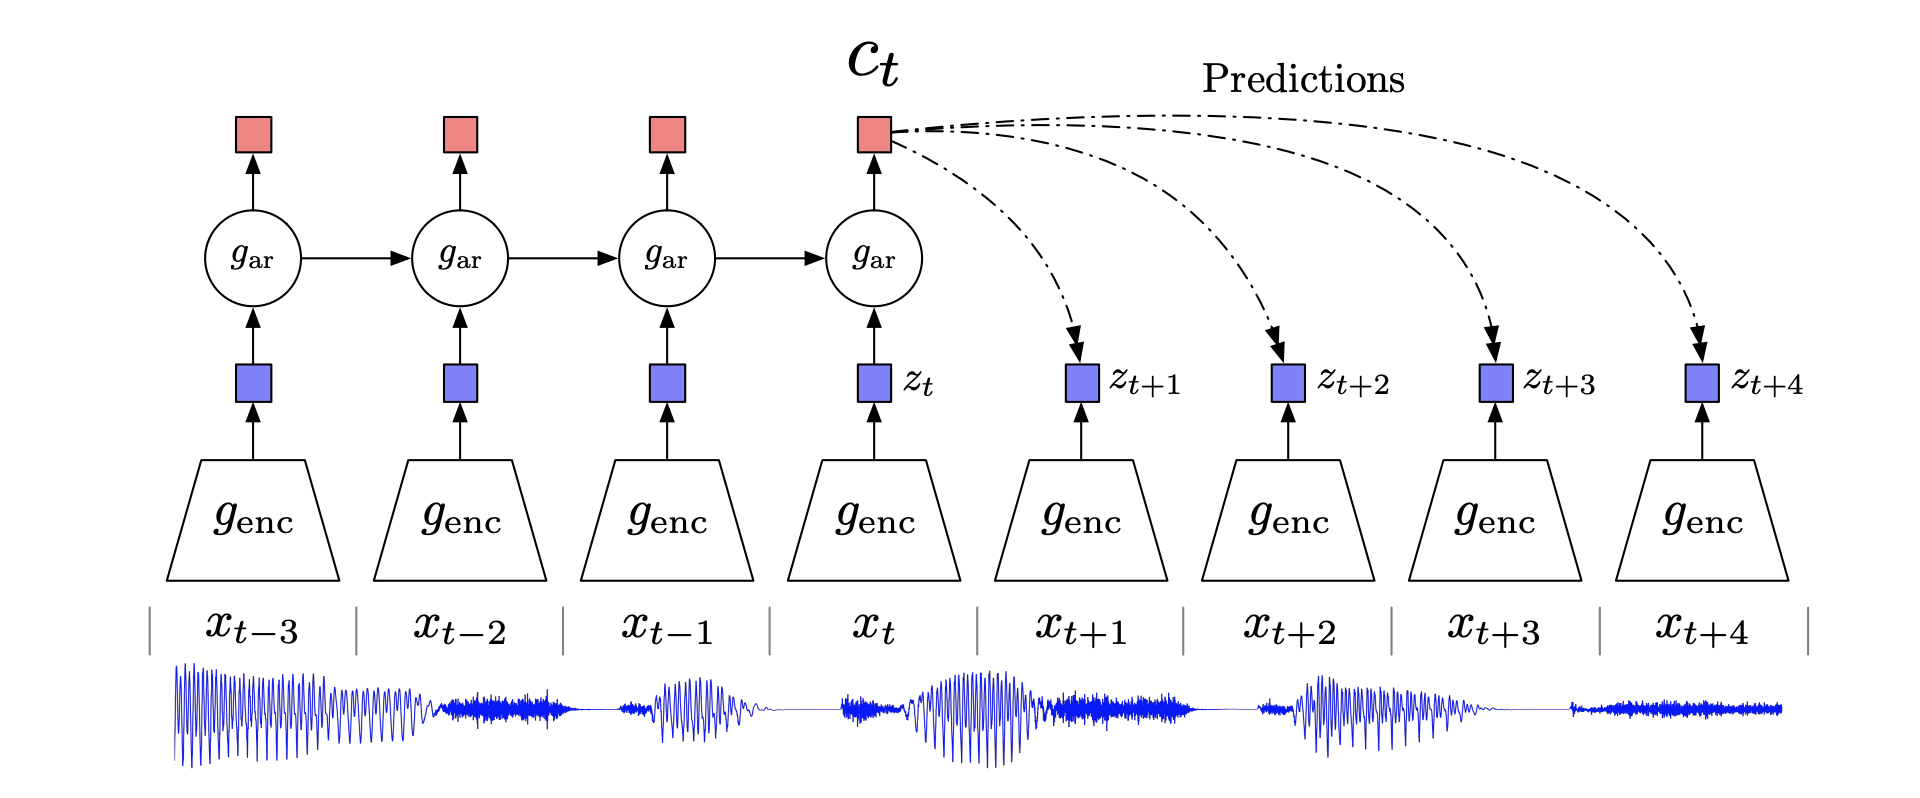
\includegraphics[width = 4.5 in]{\images/CPC}\parbox{.2in}{$z_y$ \\ \\ \\ \\ \\~}}
\vspace{-7ex}
\centerline{$|$~~~~~~~~$x$~~~~~~~$|$~~~~~~~~~~~~~~$|$~$y$~$|$}

\vfill
Consider a population distribution on pairs $\tuple{x,y}$.

\vfill
We are interested in extracting latent variables $z_x$ and $z_y$ from $x$ and $y$ respectively that preserve the mutual information between $x$ and $y$.

\slide{Mutual Information Coding General Formulation}

For a population on $\tuple{x,y}$ we introduce latent variables $z_x$ and $z_y$ defined by
mappings $z_x(x)$ and $z_y(y)$ where these mappings are defined by parameters $\Phi_x$ and $\Phi_y$ respectively.

\begin{eqnarray*}
\Phi_x^*,\Phi_y^* & = & \argmax_{\Phi_x,\Phi_y} \; I(z_x,z_y)
\end{eqnarray*}

This has a degenerate solution of $z_x(x) = x$ and $z_y(y) = y$ but this can be avoided with various types of restrictions on $z_x$ and $z_y$
as described below.

\slide{Contrastive Predictive Coding (CPC)}

\vfill
For $z_x$ and $z_y$ vectors, and for $N \geq 2$, we define a distribution on tuples $(z_x,z_{y}^1,\ldots,z_y^N,i)$
by drawing pairs $(x_1,y_1), \ldots (x_n,y_n)$ from the population, and $i$ uniformly from $1$ to $N$,
and constructing
$$(z_x(x_i),z_y(y_1),\ldots,z_y(y_N),i).$$

\vfill
We then train a model to predict $i$.
\vfill
{\huge
\begin{eqnarray*}
\Phi^* & = & \argmin_\Phi \;E_{(z_x,z_y^1,\ldots,z_y^N,i)}\left[-\ln P_\Phi(i|(z_x,z_y^1,\ldots,z_y^N)\right]
\end{eqnarray*}

\begin{eqnarray*}
P_\Phi(i|z_x,z_y^1,\ldots z_y^N) & = & \softmax_i\; z_x^\top z_y^i
\end{eqnarray*}
}

\slide{The CPC Theorem}

For any distribution on pairs $(z_x,z_y)$, if CPC probabilities are computed by

{\huge
\begin{eqnarray*}
P_\Phi(i|z_x,z_y^1,\ldots z_y^N) & = & \softmax_i\;s(z_x,z_y^i)
\end{eqnarray*}
}

then

{\huge
\begin{eqnarray*}
I(z_x,z_y) & \geq & \ln N - \;\;E_{(z_x,z_y^1,\ldots,z_y^N,i)}\left[-\ln P_\Phi(i|(z_x,z_y^1,\ldots,z_y^N)\right]
\end{eqnarray*}
}

Chen et al., On Variational Bounds of Mutual Information, May 2019.


\slide{The CPC Restriction on $z_x(x)$ and $x_y(y)$}

{\huge
\begin{eqnarray*}
P_\Phi(i|z_x,z_y^1,\ldots z_y^N) & = & \softmax_i\; z_x^\top z_y^i
\end{eqnarray*}
}

\vfill
By only using $z_x$ and $z_y$ in inner products at the final layer we force the features
to carry information in a shallow (linear) representation.

\slide{Contrastive Predictive Coding for Images}

(SimCLR:) A Simple Framework for Contrastive Learning of Visual Representations, Chen et al., Feb. 2020 (self-supervised leader as of February, 2020).

\vfill
They construct a distribution on pairs $\tuple{x,y}$ defined by drawing an image from ImageNet and then drawing $x$ and $y$ as random ``augmentations'' (modifications) of the image.

\vfill
The training maximizes the contrastive lower bound on $I(x,y)$.

\slide{Contrastive Predictive Coding for Images}

A resulting feature map $z_\Phi$ on images is extracted from this training.

\vfill
The feature map $z_\Phi$ is tested by using a {\color{red} linear} classifier for ImageNet based on these features.

\vfill
This is called linear probing.

\slide{SimCLR}

\centerline{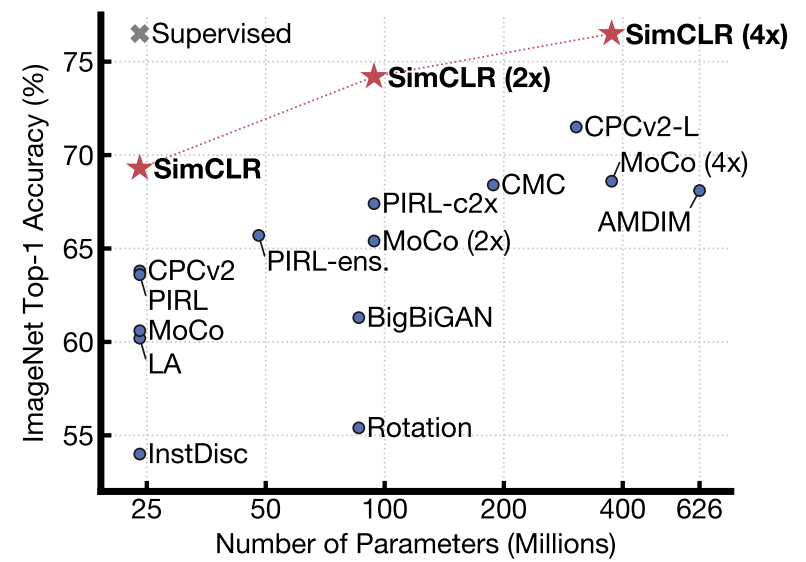
\includegraphics[height=3.5 in]{\images/SimCLR}}

\vfill
\centerline{\huge Chen et al. 2020}

\slide{A Weakness of CPC}

{\huge
\begin{eqnarray*}
I(z_x,z_y) & \geq & \ln N - \;\;E_{(z_x,z_y^1,\ldots,z_y^N,i)}\left[-\ln P_\Phi(i|(z_x,z_y^1,\ldots,z_y^N)\right]
\end{eqnarray*}
}

The discrimination problem is too easy.

\vfill
The guarantee can never be stronger than $\ln N$ where $N$ is the number of choices in the discrimination task.

\slide{Direct Mutual Information (MI) Coding}

For a population on $\tuple{x,y}$ we introduce latent variables $z_x$ and $z_y$ defined by
mappings $z_x(x)$ and $z_y(y)$ where these mappings are defined by parameters $\Phi_x$ and $\Phi_y$ respectively.

\begin{eqnarray*}
\Phi_x^*,\Phi_y^* & = & \argmax_{\Phi_x,\Phi_y} \; I(z_x,z_y) \\
\\
&= & \argmax_{\Phi_x,\Phi_y}\; H(z_y) - H(z_y|z_x) \\
\\
&= & \argmin_{\Phi_x,\Phi_y}\; H(z_y|z_x) - H(z_y)
\end{eqnarray*}

\slide{Direct MI Coding}

\begin{eqnarray*}
\Phi_x^*,\Phi_y^* & = &  \argmin_{\Phi_x,\Phi_y}\; H(z_y|z_x) - H(z_y)
\end{eqnarray*}

\vfill
We can block the solution of $z_x(x) = x$ and $z_y(y) = y$ by requiring that $z_y$ is a symbol from a limited finite vocabulary.

\vfill
This typically ensures $H(z_y) << H(y)$.

\vfill
We can then allow $H(z_x)$ to be large, for example $z_x$ might be a vector
representation of the a symbol sequence $z_1,\ldots,z_t$.

\slide{Direct MI Coding}

\begin{eqnarray*}
\Phi_x^*,\Phi_y^* & = &  \argmin_{\Phi_x,\Phi_y}\; H(z_y|z_x) - H(z_y)
\end{eqnarray*}

\vfill
If $z_y$ is a symbol from a limited vocabulary we can estimate $H(z_y)$ from an empirical histogram over the symbols.

\vfill
We can use a model $\Psi$ to predict $z_y$ from $z_x$ and train on cross-entropy loss.

\slide{Direct MI Coding}

$$\Phi_x^*,\Phi_y^*,\Psi^* = \argmin_{\Phi_x,\Phi_y,\Psi} \; E_{(x,y)\sim \pop}\left[-\ln P_\Psi(z_y|z_x) + \ln \hat{P}(z_y)\right]$$

\vfill
where $\hat{P}(z_y)$ is an estimate (perhaps an exponential moving average) of the probability of $z_y$ over the draw of $(x,y) \sim \pop$.

\slide{Direct MI Coding Theorem}

$$\Phi_x^*,\Phi_y^*,\Psi^* = \argmin_{\Phi_x,\Phi_y,\Psi} \; E_{(x,y)\sim \pop}\left[-\ln P_\Psi(z_y|z_x) + \ln P(z_y)\right]$$

\vfill
\begin{eqnarray*}
I(z_x,z_y) & \geq & H(z_y) - \hat{H}(z_y|z_x) \\
\\
\hat{H}(z_y|z_x) & = & E_{(x,y)\sim \pop}\left[-\ln P_\Psi(z_y(y)|z_x(x)\right]
\end{eqnarray*}

\slide{Direct MI Coding Theorem}

For $H(z_y) = \ln K$ where $K$ is the number of symbols, and $\hat{H}(z_y|z_x) = 0$ we get

$$I(z_x,z_y) \geq \ln K$$

\vfill
Which typically improves significantly on the best possible bound $I(z_x,z_y) \geq \ln N$ from CPC.

\slide{ SwAV}

SwAV uses direct MI coding rather than SimCLR's CPC.


\centerline{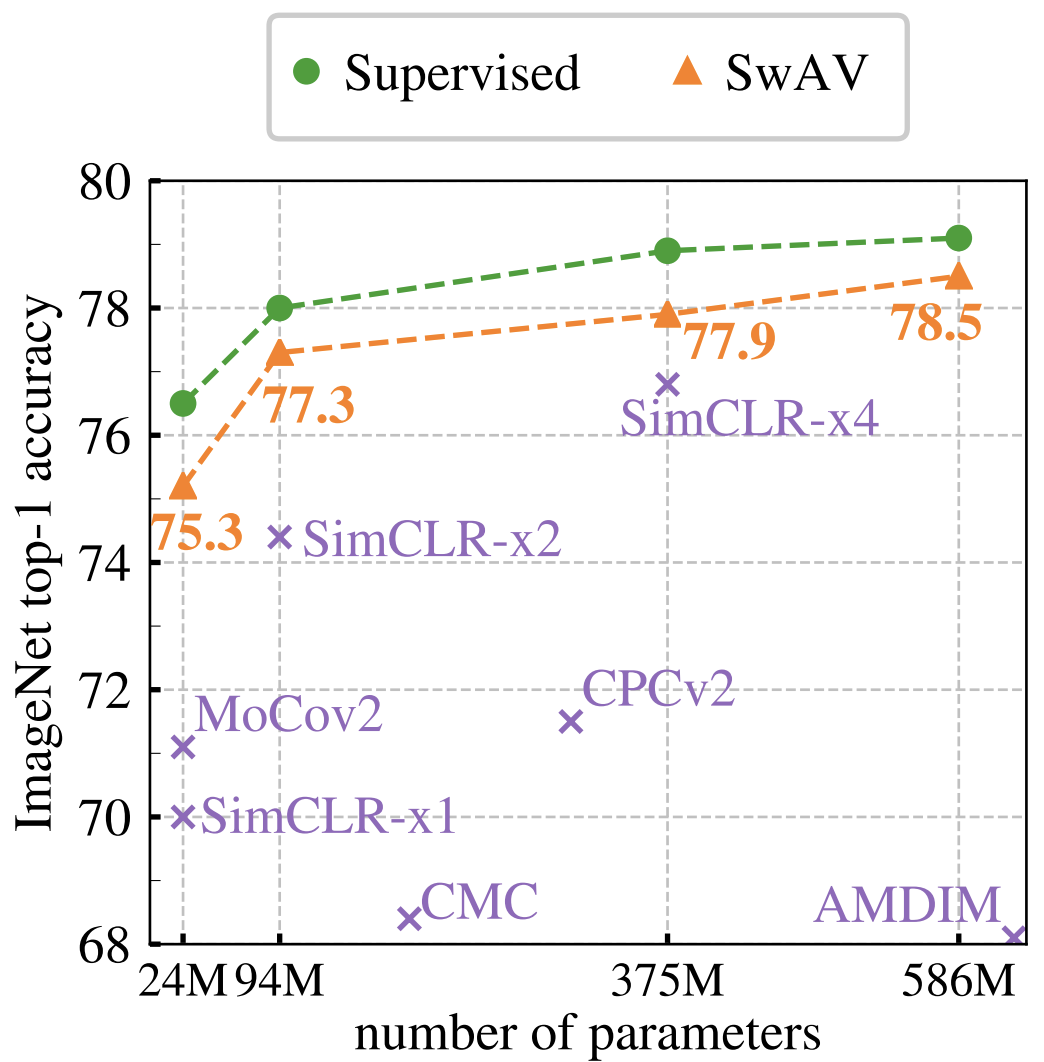
\includegraphics[width = 3.5in]{\images/SwAV}}

\centerline{\huge Caron et al. 2021}

\slide{END}

}
\end{document}


\slide{END}

}
\end{document}

